Analysis of impact craters on bodies within the solar system can give insight into properties of meteoroids forming these craters.
While there are empirical relationships for estimating the size of a crater from impactor properties and vice versa \citep[e.g.][]{holsapple1987scaling}, these relationships are not directly applicable to small impacts on planets with an atmosphere.
When impacting these planets, small-sized meteoroids experience significant deceleration, mass loss due to ablation, and potential break up before impacting the ground.
As a result of these processes, they typically produce clusters of impact craters, or only leave a strewn field of small meteorites if most of their kinetic energy has been deposited in the atmosphere.

A popular way of modeling the processes of atmospheric entry is to build on the standard meteor physics equations of motion and ablation \citep[e.g.][]{opik1958physics}, which are a set of ordinary differential equations (ODEs) treating the meteoroid as a homogeneous, spherical or ellipsoidal body.

The aim of this project is to invert impactor properties from data in a recent survey of Martian impact crater clusters \citep{daubar2019recently}.
We will investigate whether stochastic inversion methods, such as Markov Chain Monte Carlo (MCMC), are a viable approach for this problem.
MCMC models, such as the Gibbs sampler combined with the Metropolis-Hastings algorithm \citep{gelfand1990sampling}, have been a very popular black box inversion method in many research areas \citep[e.g., in epidemiology][]{flaxman2020estimating}.
In order to use an MCMC method, a high-performance numerical model of atmospheric descent and crater cluster formation is needed.


Break up is modeled to occur when the pressure difference between the leading edge and the trailing edge of the meteoroid exceeds the aerodynamic strength of the meteoroid material.
% The pressure at the leading edge, behind the bow shock, is called the stagnation pressure. The pressure on the other end, in the meteoroid wake, is nearly zero \citep{passey1980effects}.
The exact mechanism of break up is subject to ongoing research. Most break up models use either a ``pancake'' approach, or a discrete fragmentation approach \citep{register2017asteroid}.
% \cite{hills1993fragmentation} for example used a pancake approach to model energy deposition and airburst damage for various impactors on Earth. The discrete fragmentation approach was used for example by \cite{passey1980effects} to investigate strewn fields on Earth.

More recently, a combination of the two approaches, called the fragment-cloud model (FCM), was proposed by \cite{wheeler2017fragmentcloud}.
The concept behind this model was first presented by \cite{mehta2015break}.
It combines the separate-wake fragments model \citep{passey1980effects,artemieva1996interaction} with a pancake-like model:
When the meteoroid's strength is exceeded, it splits into a debris cloud plus several discrete fragments, which are all treated independently from each other after separation.
In a subsequent publication, \cite{wheeler2018atmospheric} extended their model (cf.~fig~\ref{fig:FCMv2}) and were able to demonstrate excellent agreement between simulated energy deposition and that inferred from light curves of four recent meteoroid impacts on Earth.
% They extended their FCM from the previous publication, enabling it to represent meteoroids with varied initial structures, such as rubble piles or fractured bodies. Their model was the first to successfully replicate spikes in the energy deposition curves, representing flashes in the light curve observations that they studied.

\begin{figure*}[htbp]
    \centering
    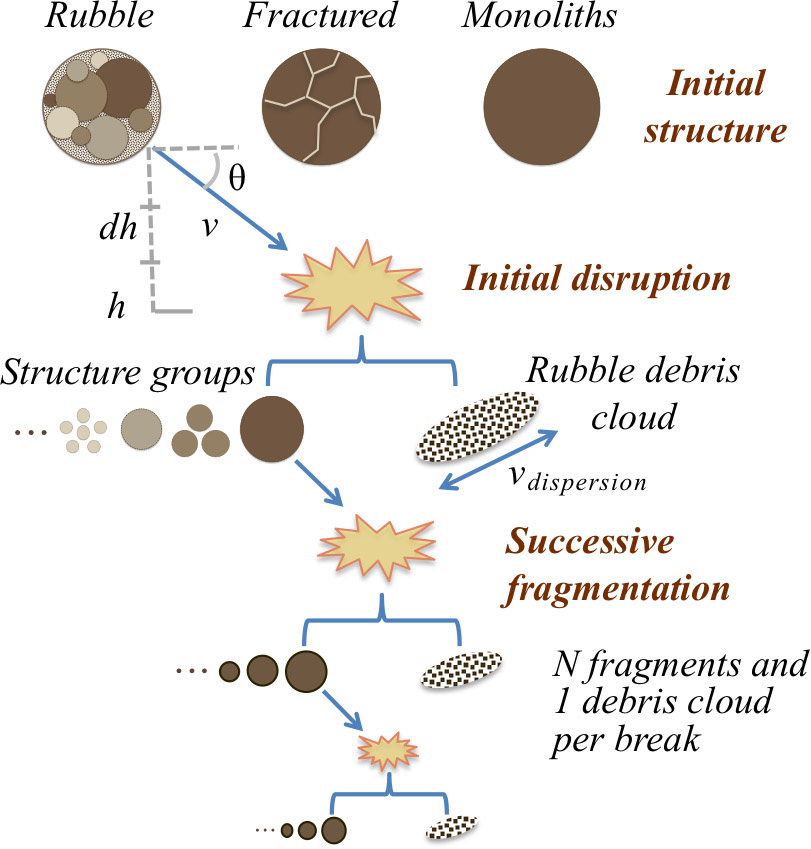
\includegraphics[width=0.7\textwidth]{figures/wheeler_diagram.jpg}
    \caption{FCM model diagram, taken from \cite{wheeler2018atmospheric}.
        A meteoroid is modeled to enter a planetary atmosphere with a speed $v$ and a trajectory angle $\theta$ relative to the ground. When the ram pressure exceeds its aeordynamic strength at height $h$ above the ground, it fragments into different structural groups, and a debris cloud. The debris cloud is described with a ``pancake''-style model. The fragments descend further into the atmosphere and may undergo successive fragmentation when their aerodynamic strength is exceeded.\label{fig:FCMv2}}
\end{figure*}

\cite{newland2019CFM18} applied the FCM model and key conclusions from the \cite{wheeler2018atmospheric} paper to the formation of impact crater clusters on Mars.
They were able to demonstrate that the FCM model, with the right parameters, was able to reproduce crater clusters with a similar distribution of certain characteristics compared to observations collected by \cite{daubar2019recently}.
They also showed that simpler models, like the discrete fragmentation approach or the FCM model without varied initial structures, as first proposed by \cite{wheeler2017fragmentcloud}, were unable to reproduce the observed distributions of cluster characteristics.

Based on these promising results, we will use the FCM model for our inversion problem.
However, a key downside of MCMC inversion methods is their heavy computational costs.
They typically run the underlying model thousands of times to generate an accurate input space distribution.
In our case, the underlying FCM model is computationally demanding in its own right.
Equations for potentially hundreds of fragments and debris clouds have to be solved numerically for each impact.

The FCM implementation by \cite{newland2019CFM18} was based in pure Python.
A single simulation run took on the order of seconds to tens of seconds, and was limited, by nature of its pure Python implementation, to be single-threaded.
To facilitate fast iteration and realistic, scalable run times for the inversion problem, we aim to develop an open source FCM implementation in a fast, compiled language, C++, along with a Python API.
We expect the performance to increase by at least two orders of magnitude from this switch on its own.
If time permits, we will investigate further optimisations.
